% Compiler: LaTeX => PDF

\documentclass{beamer}

%%%%%%%%%%%%%%%%%%%%%%%%%%%%%%%%%%%%%%%%%%%%%%%%%%%%%%%%%%%%%%%%%%%%%%%%%%%%%%%%%%
% Pr�ambel:  Hier werden Einstellungen getroffen, die global das ganze Dokument  %
%            betreffen, sowie zus�tzliche Packete bzw. Klassen angefordert.      %
%            Im einf�hrenden Beispiel werden keine weiteren Packete geladen.     %
%%%%%%%%%%%%%%%%%%%%%%%%%%%%%%%%%%%%%%%%%%%%%%%%%%%%%%%%%%%%%%%%%%%%%%%%%%%%%%%%%%

% Einbindung weiterer Packete f�r...
% ... 
\usepackage[ngerman]{babel}
% ... eine deutsche Sprachanpassung
\usepackage[latin1]{inputenc}
\usepackage{graphicx}

% \title{} Titel des Vortrages
% Anmerkung: Ohne Einbindung der Klasse "inputenc" verwendet Latex f�r Umlaute den Befehl der Form \"{<a|e|i|o|u>}
\title{Shape from X}
\subtitle{X $\in \{$ Motion, Shading, Texture $\}$}
% \author{} Name der Referenten / der Referentin
\author{Dennis Wagner\\Johannes Spangenberg\\Leroy Kramer} 
% \date definiert das Datum, das auf der Titelseite erscheinen soll \date{18. Mai 2009}
% \today f�gt das zum Zeitpunkt des LaTeX-Laufs aktuelle Datum ein.
\date{04.12.2014} 

% Mit \setbeamertemplate{footline}[<options>] l�sst sich das Aussehen der Fu�zeile �ndern.
% <options> = frame number f�gt die Folienzahl ein
\setbeamertemplate{footline}[frame number]

% \begin definiert den Beginn einer neuen Umgebung. 
% (hier: document, nach der Pr�ambel der Hauptteil eines Latex-Dokuments) 
\begin{document}
% Mit \begin{frame} <Inhalt der Folie> \end{frame} oder \frame{ <Inhalt der Folie> } erzeugt man eine neue Folie.
% \titlepage erzeugt aus den in der Pr�ambel definierten Informationen eine Titelseite. 
\frame{\titlepage} 

% \tableofcontents genieriert aus den \section und \subsection-Befehlen ein Inhaltsverzeichnis
\begin{frame}
    \frametitle{Gliederung}\tableofcontents
\end{frame} 


% \section{Name} generiert einen neuen Abschnitt
\section{Motivation} 
\frame{
    % \frametitle{} Titel der Folie
    \frametitle{Shape from X} 
    \framesubtitle{Motivation}
}


\section{Shape from Texture}
\frame{
    \frametitle{Shape from Texture}
    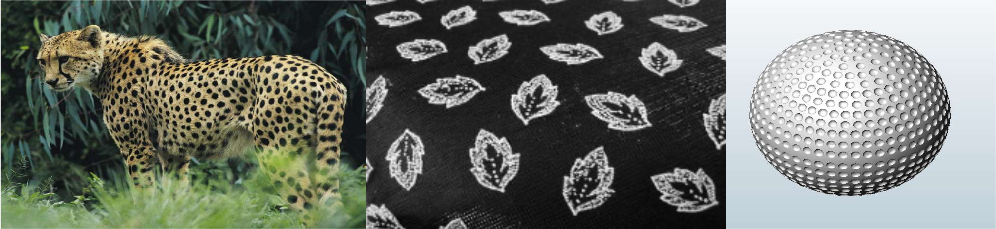
\includegraphics[width=300px, height = 69px]{sft_texture.png}\\
    
    Rekonstruktion eines 3D Objektes mit texturierter Oberfl�che aus einem Bild\\
    Textur besteht aus sich wiederholenden Texturelementen (Texel)\\
    Unterscheidung zwischen globalen und lokalen Verfahren
    
}

\frame{
    \frametitle{Shape from Texture}
    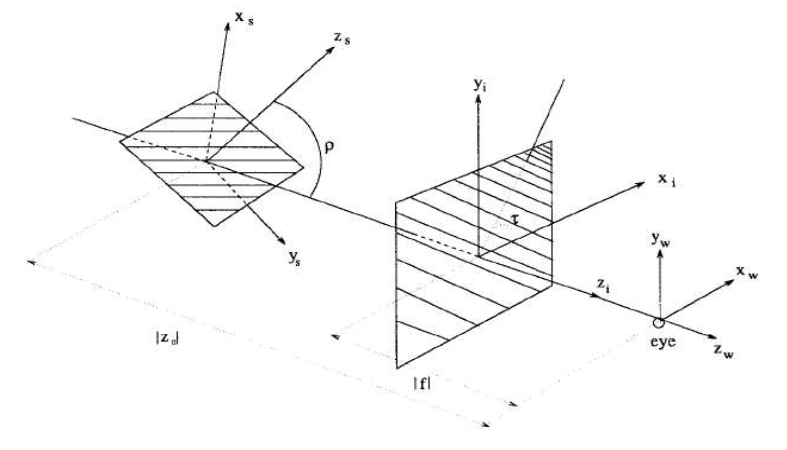
\includegraphics[width=230px, height = 120px]{sft_slant-tilt.png}\\
    
    slant $\rho$: Winkel zwischen $z_s$ und $z_i$\\
    tilt $\tau$: Winkel zwischen Projektion von $z_s$ auf Bildebene und $x_i$\\
    Normale: $n = \begin{pmatrix}
    \sin \rho \cos \tau\\
    \sin \rho \sin \tau\\
    \cos \rho
    \end{pmatrix}$
}

\frame{
    \frametitle{Shape from Texture}
    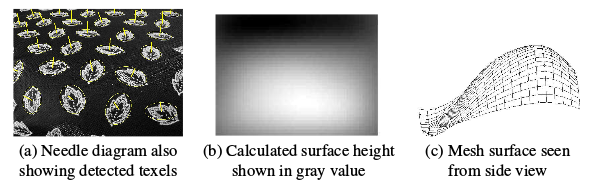
\includegraphics[width=300px, height = 96px]{sft_result.png}\\
    \vspace{1em}
    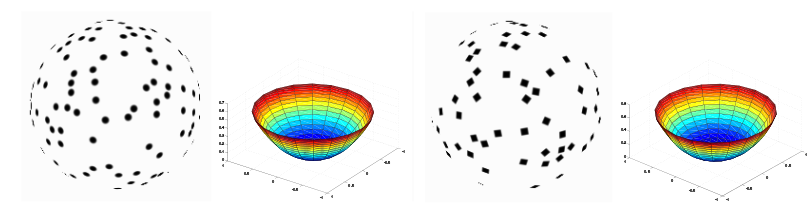
\includegraphics[width=300px, height = 81px]{sft_result2.png}\\
}

\end{document}
